\section{Methodology}
\label{sec:method}

\subsection{Conceptual Framework}

Our hypothesis is that SFT training source identity is the dominant causal factor governing
post-SFT code benchmark performance, operating through a three-step causal chain:

\textbf{Step 1:} Different code sources define distinct distributions in embedding space (tested in H-E1).

\textbf{Step 2:} SFT gradient updates bias model weights toward the training distribution (tested indirectly by H-E2's source specificity result).

\textbf{Step 3:} Performance on benchmark B is higher when the training distribution is closer to
the test distribution of B in embedding space (tested mechanistically by H-M2).

The key design insight: \textbf{token-budget equalization} isolates source identity as the sole
experimental variable, enabling causal attribution.

\subsection{Experimental Design}

We compare four SFT training source conditions on DeepSeek-Coder-Base \cite{Guo2024DeepSeekCoder}:

\begin{table}[h]
\centering
\caption{SFT training source conditions}
\label{tab:conditions}
\begin{tabular}{llrl}
\toprule
Condition & Dataset & Problems & Description \\
\midrule
HumanEval-only & openai/humaneval (train) & 164 & Algorithmic function completion with doctests \\
MBPP-only & google-research-datasets/mbpp (sanitized) & 120 & Utility scripts with I/O examples \\
LeetCode-only & newfacade/LeetCodeDataset & subsampled & Competitive programming problems \\
Equal-mix & Equal proportions from all three & --- & Structural falsifier for diversity \\
\bottomrule
\end{tabular}
\end{table}

\subsection{Token-Budget Equalization}

All four conditions receive the same effective token budget through unique-problem count $\times$
repetition rate balancing. HumanEval-only (164 problems) uses more epochs; LeetCode-only
subsamples from a larger pool. Without equalization, performance differences could reflect
data quantity rather than source identity.

\subsection{Deduplication Protocol}

We apply the validated deduplication pipeline: all-MiniLM-L6-v2 encoder, cosine similarity
threshold $>$ 0.95, against both HumanEval+ and MBPP+ test sets. Any training problem with
cosine similarity $>$ 0.95 to a test problem is removed, ensuring pass@1 differences reflect
generalization rather than memorization.

\subsection{Supervision Format Normalization}

A standardized instruction template is applied across all sources, eliminating format as
a confounding variable. All conditions use:

\begin{verbatim}
[INSTRUCTION]
Complete the following Python function.

[CODE]
{problem_prompt}
\end{verbatim}

\subsection{Distributional Alignment Measurement}

We measure embedding-space similarity between each training source and each test benchmark
using two complementary encoders:

\begin{itemize}
\item \textbf{CodeBERT} (\texttt{microsoft/codebert-base}): code-pretrained, captures programming syntax/semantics
\item \textbf{all-MiniLM-L6-v2}: sentence-level, captures problem description style
\end{itemize}

For each (source, benchmark) pair, we compute mean pairwise cosine similarity between all
source embeddings and all test benchmark embeddings. The 4$\times$2 similarity matrix per encoder
enables ranking conditions by alignment.

Figure~\ref{fig:heatmaps} shows both matrices. MiniLM shows clearer separation (range 0.247--0.311) than
CodeBERT (0.909--0.975), reflecting that problem description style diverges more than
code-level syntax.

\begin{figure}[h]
\centering
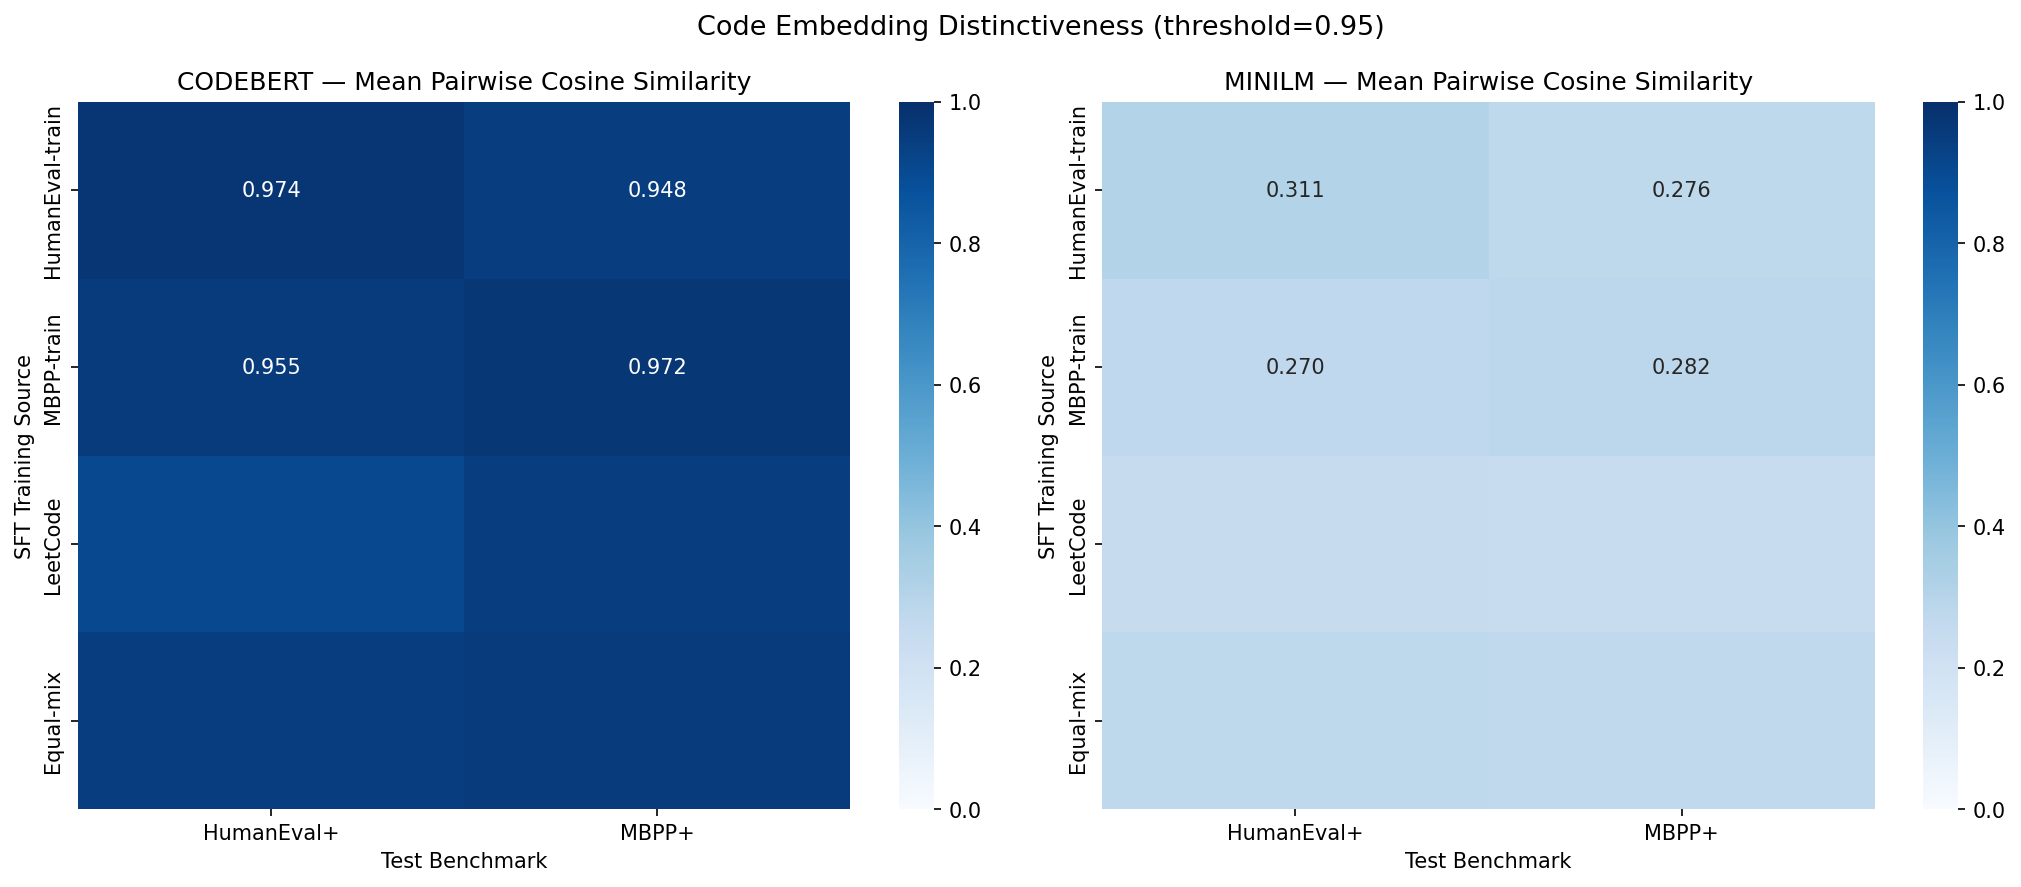
\includegraphics[width=\linewidth]{figures/similarity_heatmaps.png}
\caption{CodeBERT (left) and MiniLM (right) cosine similarity between training sources
and test benchmarks. Both confirm distinct distributions; MiniLM shows stronger separation.}
\label{fig:heatmaps}
\end{figure}

\subsection{Mechanistic Alignment Test}

Spearman $\rho$ between embedding similarity rank and pass@1 rank is computed for each
(encoder, benchmark, scale) cell. Statistical significance: permutation test, 10,000 shuffles,
one-sided (alternative: greater). Dual-encoder concordance (both encoders showing $\rho > 0$)
required for mechanistic validation.

\subsection{Training Configuration}

\textbf{1.3B:} \texttt{deepseek-ai/deepseek-coder-1.3b-base}, AdamW lr=2.0e-5, effective batch size 16,
cosine schedule, 5\% warmup, bfloat16, completion-only loss, 3 seeds (42, 123, 777).

\textbf{7B:} \texttt{deepseek-ai/deepseek-coder-7b-base}, 4-GPU DeepSpeed ZeRO-3, lr=2.0e-5, 3 epochs,
effective batch size 32, 3 seeds.

\textbf{Evaluation:} EvalPlus \cite{Liu2023EvalPlus}, greedy decoding (temperature=0).
